\chapter{Progress}

\section{Project progress}
The project has two part, currently the progress are at the point of discovering and implementing machine learning for modeling the arbiter PUF. Methods such as reinforcement learning
and graph attention neural network(so called GAT) were used. First, the type of reinforcement learning that was implemented is the SARSALambda Q learning \cite{Reference9}. The general idea is that an agent will 
explore the environment with a final goal by randomly choosing actions space and recording the rewards. 

Assuming Figure \ref{fig:figure11} is the PUF environment, red and green circle is the starting point for top path and bottom path, each black rectangle represents a multiplexer with unique delay and the yellow 
circle is the goal. There are three actions: going up, going down and going straight. The reward of multiplexer is determined by the delay, bigger the delay, the smaller the reward, vice versa. In training phase, 
the agent will travel through different combination of multiplexers and construct a Q table(See Table \ref{tab:table1}) by collecting reward on multiplexer. The final gaol for the agent is to find the route with 
lowest delay. After the training, when select a CRPs, and input the challenge to the agent, ideally, the agent can calculate, compare two paths' reward and reply the correct response. For example, challenge 00001
gives a following reward for two paths:
\begin{equation}
    Challenge(00001) =\begin{cases}
    0.082+0.008+0.041+0.002+0.07 = 0.203, & \text {Top path: 1,3,5,7,10}.\\
    0.022+0.415+0.222+0.555+0 = 1.214, & \text {Bottom path: 2,4,6,8,9}.
    \end{cases}
\end{equation}
In general, the route with lower delay will have higher reward, on the other hand, the route with higher delay will have lower reward. If the agent can predict with high accuracy, the arbiter PUF's CRPs pattern can said to 
be modelled. However, the accuracy for this modeling is around 60\% - 69\%, which is not a satisfying result. The problem can be the following: not providing enough features, the exploration does not cover every 
possible routes, etc.

\begin{figure}[htp]
    \centering
    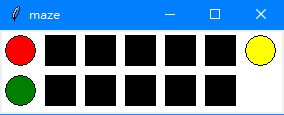
\includegraphics[width=6cm]{figures/figure11.jpg}
    \caption{SARSALambda Q learning example environment}
    \label{fig:figure11}
    \end{figure}

\begin{table}[ht]
    \center
    \begin{tabular}{c|ccc}
    Multiplexer & go up & go down & go straight\\
    \hline
    1 & 0.000 & 0.028 & 0.082\\
    2 & 0.094 & 0.000 & 0.022\\
    3 & 0.000 & 0.357 & 0.008\\
    4 & 0.009 & 0.000 & 0.415\\
    5 & 0.000 & 0.181 & 0.041\\
    6 & 0.042 & 0.000 & 0.222\\
    7 & 0.000 & 0.641 & 0.002\\
    8 & 0.003 & 0.000 & 0.555\\
    9 & 0.000 & 0.070 & 0.000\\
    10 & 0.000 & 0.000 & 0.131\\
    \end{tabular}
    \caption{Q table for example environment}
    \label{tab:table1}
    \end{table}

As for the GAT, there are some problem that need to solve. The basic idea of the GAT is that the ////. (give image!!)


In the future, XGBoost was a new idea to try if both the previous machine learning fail to model the arbiter PUF. However, more research on XGBoost was required.



